\section*{20/02/2019}
En la primera reunión realizada el martes 29 de enero del 2019 se marcaron los objetivos de plantear un tema para el trabajo. La idea original, realizar un trabajo relacionado con simulaciones que implicarán un modelo cosmológico que incorporase materia oscura caliente fue descartado debido a que el tiempo de las simulaciones sería muy superior al disponible para la entrega del trabajo. Por ello el tutor presento dos artículos de los cuales podrían sacar ideas a tratar en este trabajo. Sin embargo he encontrado otro tema que pueda ser interesante, si el tutor estuviese de acuerdo y lo viese factible. En este informe para el segundo día de reunión voy a tratar los siguiente temas.
\begin{enumerate}
\item Resumen, dudas y posibles planteamientos sobre el trabajo que ha estudiado el alumno.
\end{enumerate}

\subsection*{Impossible Early Galaxy Problem}
\subsubsection*{Resumen}
El tema que propongo para el desarrollo del trabajo fin de máster, a la espera de que el tutor lo viese propio y tenga sentido, es el planteado en el artículo de \cite{steinhardt2016impossibly} de las discordancias entre el número de densidad de los halos más masivos en redshift $z>4$ estimado por la teoría del colaps elipsoidal de \cite{10.1046/j.1365-8711.2001.04006.x}, que extiende la idea del modelo esférico de Press \& Sechter,  con las estimadas de los estudios \textit{Cosmic Assembly Near-infared Deep Extragalactic Survey} \citep[CANDELS]{grogin2011candels} y \textit{Spitzer Large Area Survey with Hyper-Suprime-Cam} \citep[SPLASH]{capak2012splash}. El primero de ellos es un estudio sobre un área del cielo mucho más pequeña pero más profunda, centrado en buscar galaxias poco masivas y así complementar los datos hasta la fecha que no permitían generar estimaciones fiables del la densidad de los halos por su masa. Mientras que el segundo estudio sobre una área del cielo mucho mas extensa, dedicada a buscar galaxias más masivas. Con los datos generados por estos estudios, \cite{steinhardt2016impossibly} estima el número de densidad de halos en función de su masa y redshift mediante tres métodos distintos.
\begin{enumerate}
\item Métodos de \textit{clusterización}, donde infieren la masa del halo por la distribución espacial de las galaxias del halo. Según \cite{steinhardt2016impossibly} estos métodos presentan la ventaja de que en simulaciones no se requiere asumir propiedades físicas de las galaxias solo la distribución materia oscura dada por el modelo cosmológico. 
\item Otra manera de inferir la masa del halo es a través de la masa estelar del halo. A través de la relación sacada en redshift más bajos \citep{leauthaud2011new} $M_H/M_\star \sim 70$.
\item El último método se basa en medir la función de luminosidad en la banda UV, sacar la relación luminosidad-masa estelar y con ella sacar la relación masa halo- masa estelar con la relación del método anterior. Mediante este método se llega a la relación $M_H / M_\odot \sim 120L_{UV} / L_\odot$.
\end{enumerate}

Comparando las estimaciones realizadas con los métodos anteriores con las predicciones teóricas de la función de masa del halo por HFMCalc \cite{murray2013hmfcalc} basadas en \cite{10.1046/j.1365-8711.2001.04006.x} se observa que existen grandes diferencias entre la teoría y las observaciones en el número de densidad de halos masivos, donde las observaciones dan una mayor densidad que lo que predice a teoría como se observa en la \textbf{Figura \ref{fig:halmf}}.
\begin{figure}
\begin{center}
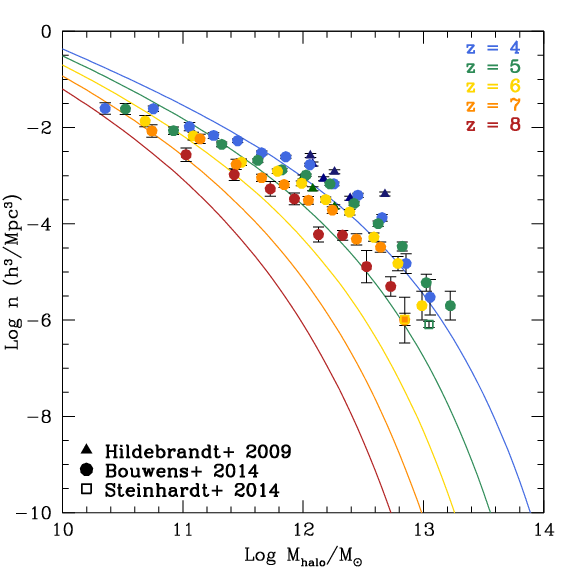
\includegraphics[scale=0.5]{Figuras/halomf}
\caption{\label{fig:halmf} La densidad teórica del número de halo en función de la masa del halo y el redshift \citep{murray2013hmfcalc} para la mayoría de los halos masivos en $4 <z <10$ (mostrados como líneas continuas, con colores más rojos con un mayor redshift) en comparación con el número en densidad de las masas de halo estimadas observacionalmente correspondientes a las galaxias de formación estelar observadas en redshifts similares. Las masas de halo se estiman usando el método de \textit{clusterización} (triángulo), mediante la masa estelar observada con la relación $M_H/ M_\star \sim 70$ (cuadrada), y mediante las luminosidades UV que se convierten en masas de halo (círculo ) con la relación $M_H / M_\odot \sim 120L_{UV} / L_\odot$. Todos estos métodos dan densidades numéricas coherentes que no están de acuerdo con las expectativas teóricas.}
\end{center}
\end{figure}

Dada que las observaciones y la teoría son inconsistentes alguna de las dos han de ser erroneas, sino las dos. Es más lógico pensar que es la teoría la que esté incompleta pero podrían también existir ciertos problemas en las estimaciones de las masa de los halos. El método en el que el artículo de \cite{steinhardt2016impossibly} parece más confiar es en el método de los ratios de masa del halo vs luminosidad en UV. Para dicho método predice dos posibles errores, uno que es común a todos los métodos es el error en la determinación del redshift de las galaxias, pero centra el error en otras fuentes. La principal fuente es que el comportamiento en los ratios de masa - luminosidad no permaneciesen constantes con los observados a redshifts más bajos. Según el desarrollo del paper implicaría un cambio muy brusco en dicho ratio a partir de z=4, lo que explica con un cambio en la IMF en redshift mayores. \\

Otras posibles explicaciones implicarían un cambio en la teoría, en donde se necesitaría un colapso de la materia barionica más temprano. Posibles soluciones pasan por plantearse otros modelos en donde cambien las limitaciones de la materia y energía oscura, como la considerancion de WDM como en \cite{gao2007gao} o el cambio del parámetro de la ecuación de estado para la densidad de energía del vacío considerando $\omega>-1$, pero según el paper entra en conflictos cuando llegamos a valores $\omega >-0.95$.\\

Por último cita la solución de que la formación estelar ocurra mucho antes que lo que se esperaría, antes del colapso inicial de los halos. Esto debería resolver primero las dfíciles limitaciones que se observan para redshift bajos y el problema del enfriamiento de pequeñas estrellas con bajas metalicidades. Sinceramente tengo grandes dudas de haberlo entendido bien pues no entiendo como es posible que la formación de estrellas llegue antes que el colapso del halo.\\

La idea es usar las simulaciones planteadas para el estudio de ete problema bajo las tres posibles soluciones que plantea el artículo y que implicaciones tendría cada una en el modelo actual de formación de galaxias y si encontraríamos algo que entrará en discordancia con lo observado hasta la fecha. Otros paper como el de \cite{yennapureddy2018cosmological} plantean un cambio en el modelo cosmológico por el modelos de $R_H=ct$ explicados en el paper \cite{10.1111/j.1365-2966.2011.19906.x} que ajustaría con mejor error las estimaciones basadas en las observaciones de CANDALS y SPLASH. (Ver \textbf{Figura \ref{fig:melia}})

\begin{figure}
\begin{center}
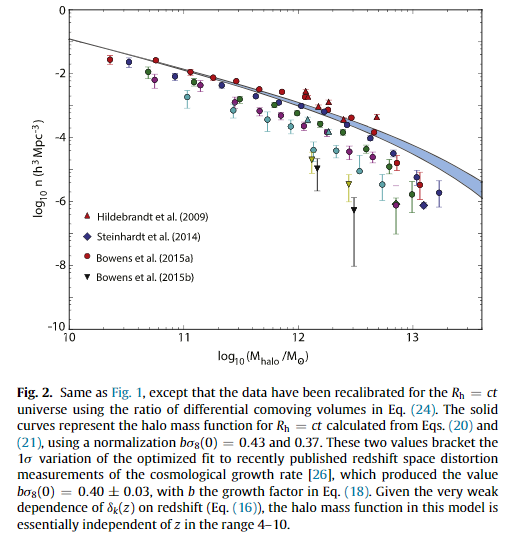
\includegraphics[scale=0.9]{Figuras/Melia}
\caption{\label{fig:melia} .}
\end{center}
\end{figure}

\subsubsection*{Planteamiento del Trabajo}

Estudio del problema planteado en el paper \cite{steinhardt2016impossibly} que me gustaría ver si estaría relacionado con el la observación de quasars a altos redshift. Ver en simulaciones que posibilidades tenemos para el estudio de este problema y hasta que punto es estudiable un cambio en el modelo cosmológico de la simulación para intentar ver como responde el problema.

\subsubsection*{Resumen de la reunión.}

Durante la reunión acordamos estudiar el tema planteado por el paper de \cite{steinhardt2016impossibly} basándonos en las tres hipótesis finales para las posibles soluciones del problema. El origen de este TFM era asarnos en simulaciones para un estudio de la formación galáctica a altos redshift pero surge un inconveniente para este tema en particular. Estudiar en simulaciones este problema requiere galaxías muy masivas a altos redshift lo que requiere, por lo primero, de un gran tiempo de simulación. El tutor no descarta darme tiempo para una simulación pero hay que estar antes muy seguro del problema a estudiar.\\

El proposito de la siguiente semana es concretar más e tema del estudio, el tutor me citó un autor \textit{Rodríguez Puebla} y el año 2018 para que busque papers relacionados y no descarta la posibilidad de hacer un trabajo puramente teoríco y dejar a futuro trabajo el llevarlo a simulaciones. El tutor plantea la posibilidad de estudiar las diferencias en simulaciones de WDM del profesor Octavio de la UNAM para introducirlas en el trabajo.
